% LaTex Template

\documentclass[12pt]{article}
\usepackage{natbib}
\usepackage[letterpaper, margin=1.1in]{geometry}
\usepackage{graphicx}
\usepackage{wrapfig}
\usepackage{enumitem}
\setlist[enumerate]{itemsep=0mm}
\usepackage{multirow}
\usepackage{lscape}
\usepackage{caption}
\usepackage{subcaption}

\begin{document}
\noindent{Alexandra Pulwicki \\ \today}

\begin{center}
\Large \textbf{Appendix\\ Density}
\end{center}

SP vs tube
snow pit ranges
tube vs depth - correction, new SP vs tube
elevation relation



\subsection*{Basic statistics}

A summary of density data collected in snowpits and when using a Federal Sampler can be seen in Table \ref{density_stats}. The standard deviation of each type of density measurement is also less than 10\% of the mean density. For snowpit derived densities, the mean density is indistinguishable between glaciers within one standard deviation. This was not observed in densities derived from Federal Sampler measurements --- Glacier 2 had the lowest mean density and Glacier 4 had the highest mean density. The mean of all Federal Sampler density values was likely skewed by the proportionally large number of measurements obtained on Glacier 13, and is thus indistinguishable from Glacier 13 mean density and different than both Glacier 4 and 2 mean density. 

\begin{table}[]
\centering
\caption{Mean, standard deviation (std), and number of measurements (n) of snow density measured on study glaciers in snowpits and using a Federal Sampler. }
\label{tab:density_stats}
\begin{tabular}{lllllll}
\begin{tabular}{ccccccc}
\multirow{2}{*}{\textbf{Glacier}} & \multicolumn{3}{c}{\textbf{Snowpits}}     & \multicolumn{3}{c}{\textbf{Federal Sampler}} \\ \cline{2-7} 
                                  & \textbf{Mean} & \textbf{Std} & \textbf{n} & \textbf{Mean}  & \textbf{Std}  & \textbf{n}  \\ \hline
\textbf{G04}                      & 348           & 13           & 3          & 360            & 10            & 7           \\
\textbf{G02}                      & 333           & 26           & 4          & 275            & 18            & 7           \\
\textbf{G13}                      & 349           & 26           & 3         & 321            & 9             & 17          \\
\textbf{All}                      & 342           & 26           & 10         & 321            & 9             & 31         
\end{tabular}
\end{table}

\subsection*{Density uncertainties}

\subsubsection*{Snowpit density}

Uncertainty in estimating density from snowpits is likely dominated by measurement errors and incorrect assumptions of density of layers that could not be sampled (i.e. ice lenses and 'hard' layers). To determine a possible range of density values from snowpit measurements, the original data was used and three parameters were varied. Ice layer density was varied between 700 and 900 kg m$^{-3}$, ice layer thickness was varied by $\pm$1 cm, and the density of layers identified as being too hard to sample (but not ice) between 600 and 700 kg m$^{-3}$. The resulting minimum and maximum possible densities for each snowpit can be seen in Table \ref{tab:density_pitrange}. The range of density values is always less than 10\% of the reference density (except for `G02\_LSP'). Density values for shallow pits that contained ice lenses were particularly sensitive to changes in density and ice lens thickness. 

\begin{table}[]
\centering
\caption{Range of snowpit density estimates. Minimum and maximum density values derived from varying ice layer density between 700 and 900 kg m$^{-3}$, ice layer thickness by $\pm$1 cm, and the density of layers identified as being too hard to sample (but not ice) between 600 and 700 kg m$^{-3}$. Reference values are those used in future analysis and were determined using an ice density of 900 kg m$^{-3}$, the recorded ice thickness, and a `hard' layer density of 600 kg m$^{-3}$.}
\label{tab:density_pitrange}
\begin{tabular}{lccccl}
\multicolumn{1}{c}{\multirow{2}{*}{\textbf{Snowpit}}} & \textbf{Density (kg m$^{-3}$)} & \textbf{} & \textbf{} & \textbf{} & \multicolumn{1}{c}{\multirow{2}{*}{\textbf{\begin{tabular}[c]{@{}c@{}}Snowpit \\ depth (cm)\end{tabular}}}} \\
\multicolumn{1}{c}{} & \textbf{Mean} & \textbf{Minimum} & \textbf{Maximum} & \textbf{Range} & \multicolumn{1}{c}{} \\ \hline
G02\_LSP & 361 & 329 & 377 & 48 & 44 \\
G02\_Z4A\_SWE & 326 & 308 & 345 & 37 & 35 \\
G02\_USP & 344 & 327 & 362 & 35 & 119 \\
G02\_ASP & 300 & 299 & 303 & 4 & 170 \\
G04\_LSP & 351 & 343 & 359 & 16 & 190 \\
G04\_USP & 333 & 317 & 350 & 33 & 160 \\
G04\_ASP & 360 & 357 & 362 & 5 & 285 \\
G13\_LSP & 383 & 383 & 383 & 0 & 20 \\
G13\_USP & 355 & 346 & 367 & 21 & 100 \\
G13\_ASP & 308 & 306 & 308 & 2 & 145
\end{tabular}
\end{table}

\subsubsection*{Federal Sampler densities}


\begin{table}[]
\centering
\caption{Range of densities estimated from Federal Sampler measurements. }
\label{my-label}
\begin{tabular}{lccccc}
\multicolumn{1}{c}{\multirow{2}{*}{\textbf{Glacier}}} & \multirow{2}{*}{\textbf{n}} & \multicolumn{3}{c}{\textbf{Density (kg m$^{-3}$)\}}} & \multirow{2}{*}{\textbf{Range as \% of mean}} \\
\multicolumn{1}{c}{} &  & \textbf{Mean} & \textbf{Minimum} & \textbf{Maximum} &  \\ \hline
G04\_Z3A\_SWE & 3 & 370 & 361 & 379 & 5 \\
G04\_USP & 6 & 352 & 328 & 364 & 10 \\
G04\_Z2A\_SWE & 3 & 368 & 353 & 377 & 7 \\
G04\_LSP & 7 & 372 & 362 & 376 & 4 \\
G04\_Z5B\_SWE & 2 & 359 & 356 & 363 & 2 \\
G04\_Z5A\_SWE & 3 & 328 & 321 & 332 & 3 \\
G04\_Z5C\_SWE & 2 & 332 & 328 & 336 & 2 \\
G02\_Z5C\_SWE & 2 & 273 & 264 & 283 & 7 \\
G02\_USP & 7 & 283 & 267 & 308 & 14 \\
G02\_Z7A\_SWE & 3 & 342 & 326 & 369 & 13 \\
G02\_Z7B\_SWE & 2 & 306 & 303 & 309 & 2 \\
G02\_Z7C\_SWE & 3 & 300 & 295 & 306 & 4 \\
G02\_Z3B\_SWE & 3 & 243 & 232 & 251 & 8 \\
G02\_LSP & 7 & 251 & 234 & 263 & 12 \\
G13\_ASP & 8 & 349 & 342 & 361 & 5 \\
G13\_651 & 3 & 352 & 344 & 367 & 7 \\
G13\_652 & 2 & 343 & 330 & 356 & 8 \\
G13\_654 & 3 & 335 & 294 & 387 & 28 \\
G13\_655 & 1 & 340 & 340 & 340 & 0 \\
G13\_656 & 3 & 336 & 313 & 363 & 15 \\
G13\_657 & 3 & 304 & 263 & 329 & 22 \\
G13\_658 & 2 & 319 & 303 & 336 & 10 \\
G13\_659 & 3 & 314 & 304 & 332 & 9 \\
G13\_Z7C\_SWE & 2 & 274 & 272 & 277 & 2 \\
G13\_USP & 6 & 317 & 301 & 331 & 9 \\
G13\_Z4C\_SWE & 1 & 408 & 408 & 408 & 0 \\
G13\_744 & 3 & 240 & 225 & 250 & 10 \\
G13\_Z3B\_SWE & 3 & 268 & 261 & 275 & 5 \\
G13\_Z4B\_SWE & 2 & 290 & 275 & 306 & 11 \\
G13\_Z5A\_SWE & 3 & 265 & 243 & 278 & 13 \\
G13\_Z5B\_SWE & 2 & 322 & 318 & 325 & 2
\end{tabular}
\end{table}

\subsection*{Comparing density from snowpit and Federal Sampler measurements}


\begin{figure}
	\centering
	\fbox{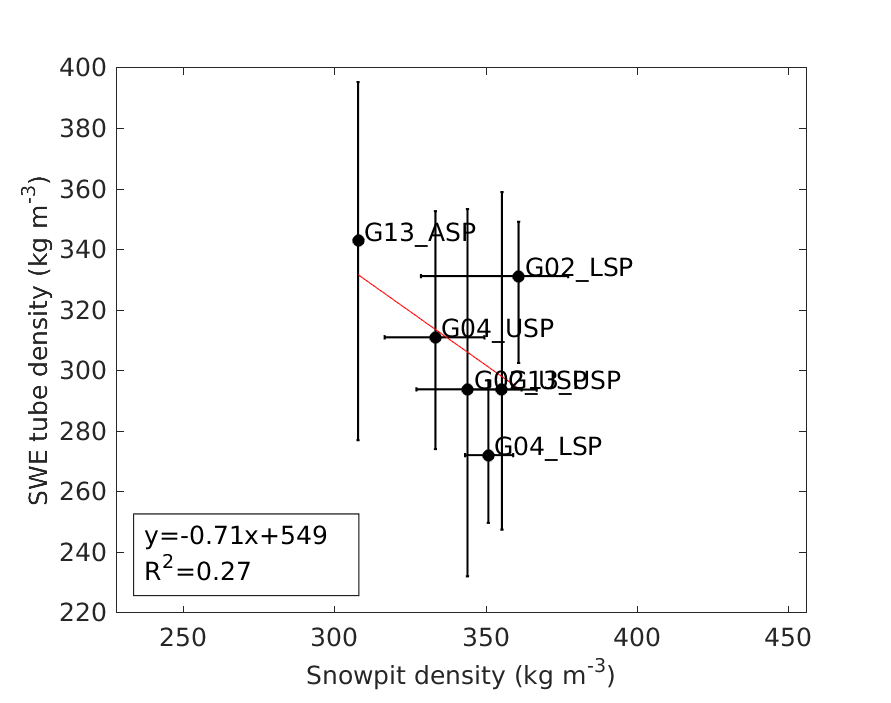
\includegraphics[\textwidth]{SnowpitVsSWEtube_all.png}}\\
	\caption{Comparison of density estimated using wedge cutters in a snow pit and Federal Sampler measurements for three study glacier (G04, G02, G13).}
	\label{fig:density_pitVStube}
\end{figure}




\begin{enumerate}
\item 
\end{enumerate}










\end{document}